\documentclass{article}
\usepackage{tikz}
\usepackage{polski}
\usepackage[utf8]{inputenc}

\newcommand{\speciallabel}[2]{
\node[above] at (#1,1 + #2){Kryt. 1};
\node[below] at (#1,-1 + #2){Kryt. 3};
\node[rotate=90] at (-1.2 + #1,#2) {Kryt. 4};
\node[rotate=270] at (1.2 + #1,#2) {Kryt. 2}; 
}

\newcommand{\startcord}[7]{%
    \speciallabel{#5}{#6}
    \draw[black] (#5,#6) circle (1cm);
    \node (p1) at (#5,#1 + #6){};
    \node (p2) at (#2+#5,#6){};
    \node (p3) at (#5,-#3 + #6){};
    \node (p4) at (-#4+#5, #6){};
    \draw[color=black,fill=#7] (p1.center) -- (p2.center) -- (p3.center) -- (p4.center) -- (p1.center);
    \draw (#5,1 + #6) -- (#5,-1 + #6);
    \draw (1+#5,#6) -- (-1+#5,#6);
}

\newcommand{\startcordlines}[7]{%
    \speciallabel{#5}{#6}
    \draw (#5,1 + #6) -- (#5,-1 + #6);
    \draw (1+#5,#6) -- (-1+#5,#6);
    \draw[black] (#5,#6) circle (1cm);
    \node (p1) at (#5,#1 + #6){};
    \node (p2) at (#2+#5,#6){};
    \node (p3) at (#5,-#3 + #6){};
    \node (p4) at (-#4+#5, #6){};
    \draw[color=#7,line width = 2.5pt] (p1.center) -- (p3.center);
    \draw[color=#7,line width = 2.5pt] (p2.center) -- (p4.center);
}


\newcommand\spider[8]{%
    \def\tempa{#1}%
    \def\tempb{#2}%
    \def\tempc{#3}%
    \def\tempd{#4}%
    \def\tempe{#5}%
    \def\tempf{#6}%
    \def\tempg{#7}%
    \spidercontinued#8
}


\newcommand{\spidercontinued}[5]{%
    \speciallabel{\tempe}{\tempf}
    \draw[black] (-1+\tempe,\tempf) -- (\tempe,1+\tempf) -- (1+\tempe,\tempf)-- (\tempe,-1+\tempf) -- cycle;
    \node (p1) at (\tempe,\tempa + \tempf){};
    \node (p2) at (\tempb + \tempe,\tempf){};
    \node (p3) at (\tempe,-\tempc + \tempf){};
    \node (p4) at (-\tempd+\tempe, \tempf){};
    \draw[color=black,fill=\tempg] (p1.center) -- (p2.center) -- (p3.center) -- (p4.center) -- (p1.center);
    \draw[color = black,fill = brown!50!black] (\tempe,\tempf+#2) --  (\tempe + #3,\tempf) --  (\tempe,\tempf - #4) --  (\tempe -#5 ,\tempf) --  (\tempe,\tempf+#2);
    \draw (\tempe,1 + \tempf) -- (\tempe,-1 + \tempf);
    \draw (1+\tempe,\tempf) -- (-1+\tempe,\tempf);
}



\begin{document}


%[[594, 202, 202, 202], [608, 78, 170, 78], [646, 25, 25, 25], [647, 281, 799, 281]]

\begin{figure}[]
    \centering
    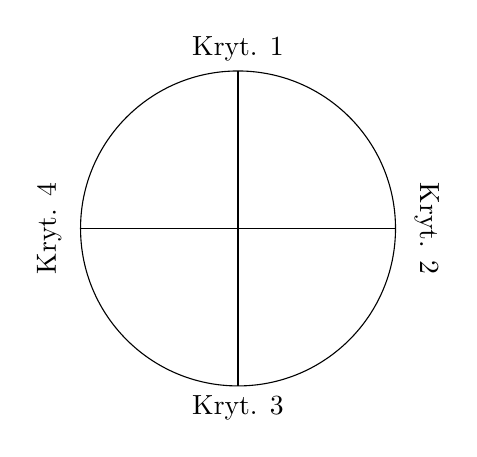
\begin{tikzpicture}[scale=2.0]
        % #1-kryt. 1 #2-kryt. 2  #3-kryt. 3  #4-kryt. 4  #5-współ. x  #6 współ. y  #7-kolor
        %\startcord{0.0}{0.875}{0.667}{1.0}{0}{0}{yellow}
        % #1-kryt. 1 #2-kryt. 2  #3-kryt. 3  #4-kryt. 4  #5-współ. x  #6 współ. y  #7-kolor
        %\startcordlines{0.0}{0.875}{0.667}{1.0}{2}{2}{red}
        % #1-kryt. 1 #2-kryt. 2  #3-kryt. 3  #4-kryt. 4  #5-współ. x  #6 współ. y  #7-kolor #8 musi być 1 #9 1-kryt obszaru nieosiągalnego #10 2-kryt obszaru nieosiągalnego #11 3-kryt obszaru nieosiągalnego #12 4-kryt obszaru nieosiągalnego
        %\spider{0.1667}{0.9}{0.750}{1.0}{4}{-1}{blue}{1}{0.16}{0.2}{0.5}{0.3333}
        \startcord{1.0}{0.0}{0.0}{0.0}{3.0}{0}{yellow}
    \end{tikzpicture}
    \caption{Wizualizacja współrzędnych gwiazdowych- rozwiązanie 1}
    \label{fig:star_cord}
\end{figure}

\begin{figure}[]
    \centering
    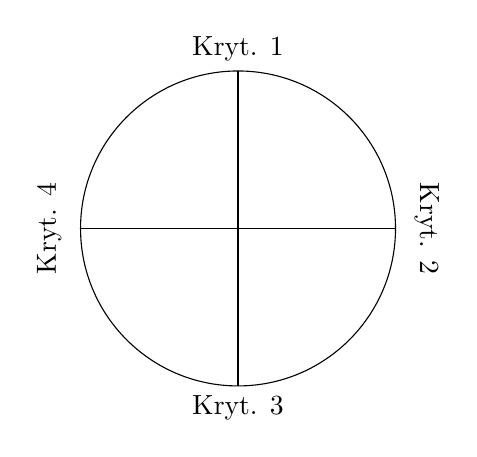
\begin{tikzpicture}[scale=2.0]
        \startcord{1.0}{0.0}{0.32}{0.0}{3.0}{0}{green}
    \end{tikzpicture}
    \caption{Wizualizacja współrzędnych gwiazdowych- rozwiązanie 2}
    \label{fig:star_cord}
\end{figure}

\begin{figure}[]
    \centering
    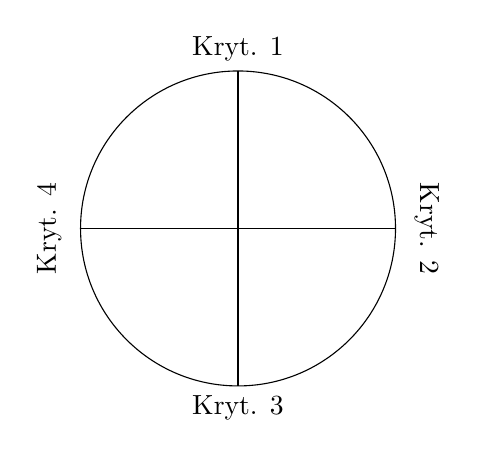
\begin{tikzpicture}[scale=2.0]
        \startcord{1.0}{0.0}{0.0}{0.0}{3.0}{0}{red}
    \end{tikzpicture}
    \caption{Wizualizacja współrzędnych gwiazdowych- rozwiązanie 3}
    \label{fig:star_cord}
\end{figure}

\begin{figure}[]
    \centering
    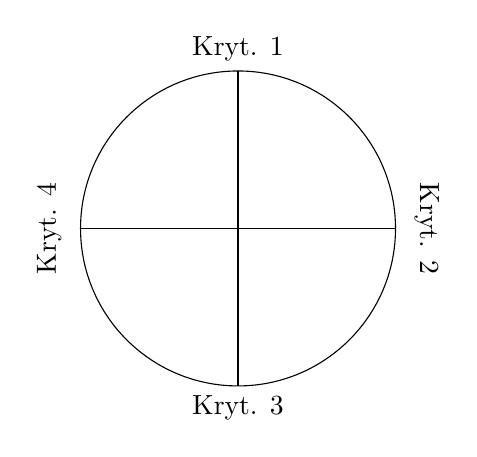
\begin{tikzpicture}[scale=2.0]
        \startcord{0.8}{0.0}{1.0}{0.0}{3.0}{0}{blue}
    \end{tikzpicture}
    \caption{Wizualizacja współrzędnych gwiazdowych- rozwiązanie 4}
    \label{fig:star_cord}
\end{figure}

\begin{figure}[]
    \centering
    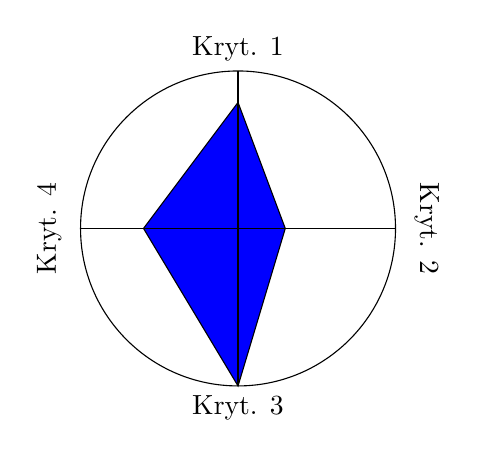
\begin{tikzpicture}[scale=2.0]
        \startcord{0.8}{0.3}{1.0}{0.6}{3.0}{0}{blue}
    \end{tikzpicture}
    \caption{Przykład wizualizacji współrzędnych gwiazdowych \linebreak (ponieważ na poprzednich wykresach nie widać możliwości wykresu)}
    \label{fig:star_cord}
\end{figure}

\end{document}
